\section{Resultados da RQ 08}

Escolhemos a opção do \textit{rework rate} e não analisamos a evolução temporal, que a hipótese da RQ 08 também previa. O \textit{rework rate} tem mediana de 31,1\% (IQR de 14,2\% a 52,5\%), e 29 repositórios o têm igual a zero. O CFR (b) tem mediana de 17,4\% (IQR de 5,9\% a 32,8\%). O \textit{rework rate} é maior que o CFR (b) em 223 dos 298 repositórios com as duas métricas, menor em 19 e igual em 56 (diferença significativa pelo teste de Wilcoxon pareado unilateral, $p < 0{,}001$, e correlação \textit{rank-biserial} de 0,97). A correlação de Spearman entre os dois é positiva e forte ($\rho = 0{,}706$; $n = 298$). A Figura~\ref{fig:rq08} mostra que a maioria dos repositórios fica acima da diagonal.

\begin{figure}[ht]
\centering
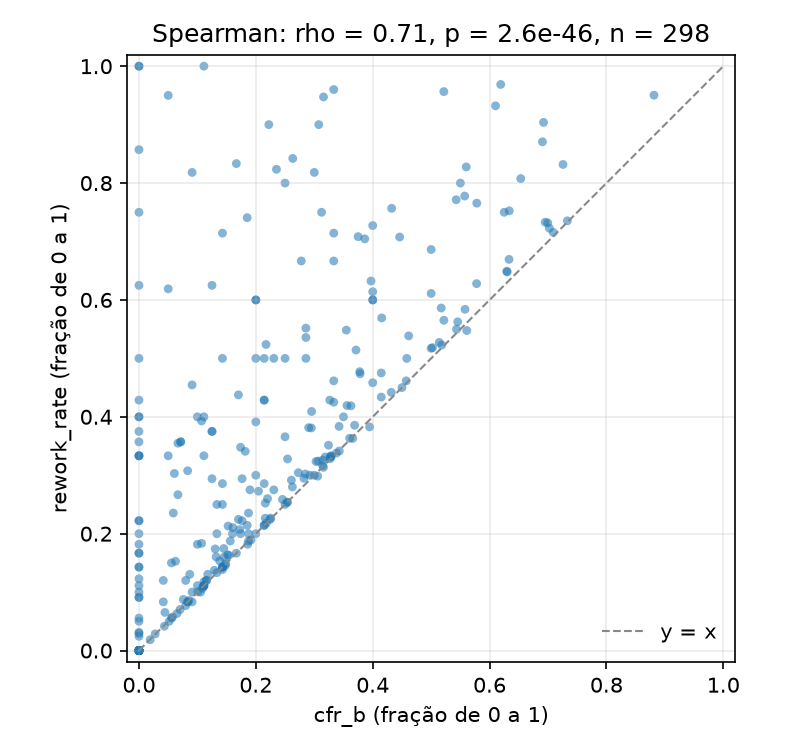
\includegraphics[width=0.55\textwidth]{rq08_cfr_b.png}
\caption{\textit{Rework rate} contra CFR (b) de cada repositório; a linha é a diagonal $y = x$.}
\label{fig:rq08}
\end{figure}

Confirmamos as três hipóteses sobre o \textit{rework rate}: a mediana fica entre 20\% e 40\%, o valor é maior que o do CFR (b) e a correlação com ele é forte. A hipótese sobre a evolução temporal ficou sem teste. O \textit{rework rate} é maior porque conta as releases corretivas publicadas depois dos 7 dias e as que corrigem outra correção, que o CFR (b) não conta, e é a métrica que o DORA adotou em 2024. A correlação forte entre os dois também tem uma causa em comum: ambos dependem da mesma heurística de release corretiva, cujo F1 é de 0,644, e herdam os mesmos erros. Por isso a correlação não prova que os dois medem o mesmo fenômeno, só que erram juntos.
